\documentclass[aspectratio=169]{beamer}
\mode<presentation>

\usepackage[T1]{fontenc}
\usepackage[utf8]{inputenc}
\usepackage{lmodern}
\usepackage[ngerman]{babel}
\usepackage{presentationST}
\usepackage{hyperref}
\usepackage{pgfplots}\pgfplotsset{compat=1.13} % necessary?
\usepackage{multimedia}
\usepackage{algpseudocode}
\usepackage{tikz}
\usetikzlibrary{patterns, calc}
\algnewcommand{\IIf}[1]{\State\algorithmicif\ #1\ \algorithmicthen}
\algnewcommand{\EndIIf}{\unskip\ \algorithmicend\ \algorithmicif}
\renewcommand{\Comment}[2][.5\linewidth]{\leavevmode\hfill\makebox[#1][l]{//~#2}}
\usepackage{floatflt} 

\hypersetup{unicode=true, pdftoolbar=true, pdfmenubar=true, pdffitwindow=false, 
	pdfstartview={FitH},
	pdftitle={Numerische Simulation: Mehrgitter und Konjugierte Gradienten Methode},
	pdfauthor={Stephan Lunowa, Jonas Harsch, Markus Baur},
	pdfsubject={Mehrgitter, Konjugierte Gradienten, Wintersemester 2016/17},
	pdfcreator={\LaTeX\ with ptextbfkage \flqq hyperref\frqq},
	pdfproducer={pdfTeX \the\pdftexversion.\pdftexrevision},
	pdfnewwindow=true,
	colorlinks=true,linkcolor=black,citecolor=black,filecolor=magenta,urlcolor=black}

%%%%%%%%%%%%%%%%%%%%%%%%%%%%%%%%%%%%%%%%%%%%%%%%%%%%%%%%%%%%%%%%%%%%%%%%%%%%
% For Printing
%%%%%%%%%%%%%%%%%%%%%%%%%%%%%%%%%%%%%%%%%%%%%%%%%%%%%%%%%%%%%%%%%%%%%%%%%%%%
%\usepackage{pgfpages}
%\pgfpagesuselayout{resize to}[a4paper,border shrink=5mm,landscape]
%Zum Drucken von 8 Folien pro Seite setzt man die Layoutoptionen entsprechend des ntextbfhfolgenden Beispiels.
%\pgfpagesuselayout{8 on 1}[a4paper,border shrink=5mm]

%%%%%%%%%%%%%%%%%%%%%%%%%%%%%%%%%%%%%%%%%%%%%%%%%%%%%%%%%%%%%%%%%%%%%%%%%%%%
% Mathematical Symbols and blocks
%%%%%%%%%%%%%%%%%%%%%%%%%%%%%%%%%%%%%%%%%%%%%%%%%%%%%%%%%%%%%%%%%%%%%%%%%%%%
\newcommand{\N}{\mathbb{N}}
\newcommand{\R}{\mathbb{R}}
\newcommand{\diff}[1]{\partial_{#1}}
\DeclareMathOperator{\divergence}{div}
\newtheoremstyle{thm}%
  {}%         Sptextbfe above, empty = `usual value'
  {}%         Sptextbfe below
  {\itshape}% Body font
  {}%         Indent amount (empty = no indent, \parindent = para indent)
  {\bfseries}% Thm head font
  {}%         Punctuation after thm head
  {\newline}% Sptextbfe after thm head: \newline = linebreak
  {}%         Thm head spec
\theoremstyle{thm}
%\newtheorem{theorem}{Satz}[section] % schon definiert
%\newtheorem{lemma}[theorem]{Lemma} % schon definiert
%\newtheorem{definition}[theorem]{Definition} % schon definiert
\newtheorem{assumption}[theorem]{Annahme}
\newtheorem{remark}[theorem]{Bemerkung}

%%%%%%%%%%%%%%%%%%%%%%%%%%%%%%%%%%%%%%%%%%%%%%%%%%%%%%%%%%%%%%%%%%%%%%%%%%%%
% Titlepage
%%%%%%%%%%%%%%%%%%%%%%%%%%%%%%%%%%%%%%%%%%%%%%%%%%%%%%%%%%%%%%%%%%%%%%%%%%%%
\title{Mehrgitter und Konjugierte Gradienten Methode}
\subtitle{Numerische Simulation}
\author{Markus Baur \and Jonas Harsch \and Stephan Lunowa}
\institute[IPVS]{Prof. Dr. rer. nat. habil. M. Mehl\\
Institut für Parallele und Verteilte Systeme\\
Universität Stuttgart}
\date{\today}

%%%%%%%%%%%%%%%%%%%%%%%%%%%%%%%%%%%%%%%%%%%%%%%%%%%%%%%%%%%%%%%%%%%%%%%%%%%%
% Document
%%%%%%%%%%%%%%%%%%%%%%%%%%%%%%%%%%%%%%%%%%%%%%%%%%%%%%%%%%%%%%%%%%%%%%%%%%%%
\begin{document}

\frame[plain]{\mbox{}\vspace{2em}\titlepage}
\frame[plain]{\frametitle{Inhalt} \setcounter{tocdepth}{1} \tableofcontents }
% framenumber neu setzen, damit Nummerierung bei 1 anfängt.
%\setcounter{framenumber}{0}

%%%%%%%%%%%%%%%%%%%%%%%%%%%%%%%%%%%%%%%%%%%%%%%%%%%%%%%%%%%%%%%%%%%%%%%%%%%%
% Mehrgitter Methode
%%%%%%%%%%%%%%%%%%%%%%%%%%%%%%%%%%%%%%%%%%%%%%%%%%%%%%%%%%%%%%%%%%%%%%%%%%%%
\section{Mehrgitter Methode}\label{sec:MG}
\begin{frame}{Mehrgitter Methode (MG)}
  \begin{itemize}[<+(1)->]
    \item Multigrid / Multilevel / Mehrgitter Methode
    \item Iterative Löser langsam für glatte Fehler
    \item Glatte Fehler auf gröberen Gittern oszillierend
    \item Mehrgitter hat $h$-unabhängige Konvergenzrate
    \item Essentiell: Beachtung der Randbedingungen um kleine Konvergenzfaktoren
        zu erhalten
    \item \textcolor{red}{\huge TODO}
  \end{itemize}
\end{frame}

\begin{frame}{Mehrgitter Methode (MG)}
  \begin{minipage}{0.49\linewidth}
  \begin{align*}
    \intertext{Im Gebiet:}
    \Delta p &= rhs + res \\
    \Delta e^c &= res^c = R_\Omega\ res
    \intertext{Analog auf dem Rand für Neumann-RB:}
    \partial_n p &= rhs + res \\
    \partial_n e^c &= res^c = R_\Gamma\ res
  \end{align*}
  \end{minipage}
  \begin{minipage}{0.49\linewidth}
  Beispiel linker Rand:\\[0.2cm]
  \begin{tikzpicture}[scale=1.0]
    \draw [step=1.0cm, pattern=north east lines, opacity=0.5] (1.0,0.0) rectangle (2.0,1.0);
    \draw [step=1.0cm, pattern=north east lines, opacity=0.5] (1.0,1.0) rectangle (2.0,2.0);
    \draw [white, step=1.0cm, pattern=north east lines, opacity=0.5] (1.0,2.0) rectangle (2.0,2.5);
    \draw [white, step=1.0cm, pattern=north east lines, opacity=0.5] (1.0,0.0) rectangle (2.0,-0.5);
    \draw[step=2.0, red, ultra thick] (0.0, -0.5) grid (4.5, 2.5);
    \draw[step=1.0, black] (0.0, -0.5) grid (4.5, 2.5);

	\foreach \i in {1.5,...,3.5} {
      \foreach \j in {0.5,...,1.5} {
        \draw[blue, fill] (\i, \j) circle[radius=0.08cm];
      }
    }

    \draw[blue] (1.5, 0.5) node[above] {\scriptsize $p_{0,j}$};
    \draw[blue] (1.5, 1.5) node[above] {\scriptsize $p_{0,j+1}$};
    \draw[blue] (2.5, 0.5) node[above] {\scriptsize $p_{1,j}$};
    \draw[blue] (2.5, 1.5) node[above] {\scriptsize $p_{1,j+1}$};

	\foreach \i in {1.0,3.0} {
      \draw[red, fill] (\i, 1.0) circle[radius=0.08cm];
    }

	\draw[red] (1.0, 1.0) node[above, xshift=-0.25cm, yshift=-0.05cm] {\scriptsize $p^c_{0,j}$};
    \draw[red] (3.0, 1.0) node[above, xshift=-0.25cm, yshift=-0.05cm] {\scriptsize $p^c_{1,j}$};

    \draw[red, ultra thick] (4.8, 1.5) -- (5.2,1.5) node[right] {\textcolor{black}{grobes Gitter}};
    \draw[black] (4.8, 0.5) -- (5.2,0.5) node[right] {feines Gitter};
  \end{tikzpicture}
  \begin{align*}
    \tfrac{p_{1,j}-p_{0,j}}{h} &= rhs_{0,j} + res_{0,j} \\
    \tfrac{e^c_{1,j}-e^c_{0,j}}{2h} &= rhs^c_{0,j} = \tfrac{1}{2}(res_{0,j+1}+res_{0,j})
  \end{align*}
  \end{minipage}
\end{frame}

%%%%%%%%%%%%%%%%%%%%%%%%%%%%%%%%%%%%%%%%%%%%%%%%%%%%%%%%%%%%%%%%%%%%%%%%%%%%
% Konjugierte Gradienten Methode
%%%%%%%%%%%%%%%%%%%%%%%%%%%%%%%%%%%%%%%%%%%%%%%%%%%%%%%%%%%%%%%%%%%%%%%%%%%%
\section{Konjugierte Gradienten Methode}\label{sec:CG}
\begin{frame}{Konjugierte Gradienten Methode (CG)}
  \begin{itemize}[<+(1)->]
    \item Minimierung von $E(x) = \tfrac{1}{2}\langle Ax, x\rangle - \langle b,x \rangle$\\
        $\qquad\Rightarrow E'(x) = Ax - b \stackrel{!}{=} 0 \qquad\text{für}\quad A$
        symmetrisch positiv definit
    \item Suchrichtung in Gradientenrichtung liefert schnelle Konvergenz
    \item Ausschöpfen des kompletten $\R^N$  durch $A$-Konjugieren
        $\langle Ad_k, d_j\rangle = 0 \ \forall k \neq j$
    \item Optimierung des Algorithmus liefert als wesentlichen Aufwand eine
        Matrix-Vektor-Multiplikation pro Iteration
  \end{itemize}
\end{frame}

\begin{frame}[fragile]{Konjugierte Gradienten Methode (CG)}
  \small
  \begin{algorithmic}
    \Function{CG}{$A,b,x_0$} \Comment{Löst das LGS $Ax = b$}
    \State $r_0 := Ax - b$ \Comment{Initiales Residuum}
    \State $d_0 := r_0$    \Comment{Initiale Suchrichtung}
    \For{$k = 0, 1, \dots$}
      \State $z := Ad_k$
      \State $\alpha_k := \frac{\langle r_k, r_k \rangle}{\langle d_k, z\rangle}$
        \Comment{Optimale Suchweite}
      \State $x_{k+1} := x_k + \alpha_k d_k$
        \Comment{Korrektur der Lösung}
      \State $r_{k+1} := r_k - \alpha_k z$
        \Comment{Korrektur des Residuums}
      \State $\beta_k := \frac{\langle r_{k+1}, r_{k+1} \rangle}{\langle r_k, r_k\rangle}$
        \Comment{$A$-Konjugiertheit}
      \State $d_{k+1} := r_{k+1} + \beta_k d_k$
        \Comment{Korrektur der Suchrichtung}
      \State // Update der Randbedingungen
      \IIf{$\|r_{k+1}\| < \varepsilon$} break \EndIIf \Comment{Abbbruchbedingung}
    \EndFor
    \EndFunction
  \end{algorithmic}
\end{frame}

%%%%%%%%%%%%%%%%%%%%%%%%%%%%%%%%%%%%%%%%%%%%%%%%%%%%%%%%%%%%%%%%%%%%%%%%%%%%
% Numerische Ergebnisse
%%%%%%%%%%%%%%%%%%%%%%%%%%%%%%%%%%%%%%%%%%%%%%%%%%%%%%%%%%%%%%%%%%%%%%%%%%%%
\section{Numerische Ergebnisse}\label{sec:Ergebnisse}
\begin{frame}{Numerische Ergebnisse}
  \begin{minipage}{0.59\linewidth}
  \begin{tikzpicture}\begin{loglogaxis}[width=8cm,
    xlabel={\#Gitterpunkte $N$ in einer Dimension}, ylabel={\#Iterationen}, grid=minor,
    log basis x=2, legend pos= outer north east,
    legend entries={MG, CG, RBSOR, SOR, $\mathcal{O}(N)$},
    domain=4:128]
    \addplot table {data/it_MG.csv};
    \addplot table {data/it_CG.csv};
    \addplot table {data/it_RB.csv};
    \addplot table {data/it_SOR.csv};
    \addplot[black, dashed] {8*x};
  \end{loglogaxis}\end{tikzpicture}
  \end{minipage}
  \begin{minipage}{0.4\linewidth}\small~\vspace{2.5cm}
    
  Parameter: \\
  $\omega$ optimal, $\gamma = 1$, $\nu = 4$, $\varepsilon = 10^{-6}$,
  zufällige identische Anfangsdaten \\$p \sim \mathcal{N}(0,1)$,
  gemittelt über 5 Läufe.
  \end{minipage}
\end{frame}

\begin{frame}{Numerische Ergebnisse}
  \begin{minipage}{0.59\linewidth}
  \begin{tikzpicture}\begin{loglogaxis}[width=8cm,
    xlabel={\#Gitterpunkte $N$ in einer Dimension}, ylabel={Laufzeit}, grid=minor,
    log basis x=2, legend pos= outer north east,
    legend entries={MG, CG, RBSOR, SOR, $\mathcal{O}(N^3)$, $\mathcal{O}(N^2)$},
    domain=16:256]
    \addplot table {data/drivencavity_1MG.csv};
    \addplot table {data/drivencavity_1CG.csv};
    \addplot table {data/drivencavity_1RBSOR.csv};
    \addplot table {data/drivencavity_1SOR.csv};
    \addplot[black, dashed] {x^3/1500};
    \addplot[black, dotted] {x^2/600};
  \end{loglogaxis}\end{tikzpicture}
  \end{minipage}
  \begin{minipage}{0.4\linewidth}\small~\vspace{2.5cm}
    
  Driven-Cavity: \\
  sequentiell mit $Re = 1000$, $\omega$ optimal, $\gamma = 1$, $\nu = 4$,
  $\alpha = 0.9$, $dt = 10^{-3}$, $T_{end} = 1$, $\varepsilon = 10^{-6}$, $\tau = 0.75$, \\
  gemittelt über 5 Läufe.
  \end{minipage}
\end{frame}

\begin{frame}{Numerische Ergebnisse}
  \begin{minipage}{0.59\linewidth}
  \begin{tikzpicture}\begin{loglogaxis}[width=8cm,
    xlabel={\#Gitterpunkte $N$ in einer Dimension}, ylabel={Laufzeit}, grid=minor,
    log basis x=2, legend pos= outer north east,
    legend entries={MG, CG, RBSOR, SOR, $\mathcal{O}(N^3)$, $\mathcal{O}(N^2)$},
    domain=16:256]
    \addplot table {data/drivencavity_2parallelMG.csv};
    \addplot table {data/drivencavity_2parallelCG.csv};
    \addplot table {data/drivencavity_2parallelRBSOR.csv};
    \addplot table {data/drivencavity_2parallelSOR.csv};
    \addplot[black, dashed] {x^3/1500};
    \addplot[black, dotted] {x^2/600};
  \end{loglogaxis}\end{tikzpicture}
  \end{minipage}
  \begin{minipage}{0.4\linewidth}\small~\vspace{2.5cm}
  
  Driven-Cavity: \\
  parallel auf 2 Prozessoren, $Re = 1000$, $\omega$ optimal,
  $\gamma = 1$, $\nu = 4$, $\alpha = 0.9$, $dt = 10^{-3}$, $T_{end} = 1$,
  $\varepsilon = 10^{-6}$, \\
  $\tau = 0.75$, gemittelt über 5 Läufe.
  \end{minipage}
\end{frame}

\begin{frame}{Numerische Ergebnisse}
  \begin{minipage}{0.59\linewidth}
  \begin{tikzpicture}\begin{semilogxaxis}[width=8cm,
    xlabel={\#Gitterpunkte $N$ in einer Dimension}, ylabel={Speedup},
    log basis x=2, legend pos= outer north east, grid=major,
    legend entries={MG (2), CG (2), RBSOR (2), SOR (2), MG (4), CG (4), RBSOR (4), SOR (4)}]
    \addplot table {data/speedup2_MG.csv};
    \addplot table {data/speedup2_CG.csv};
    \addplot table {data/speedup2_RB.csv};
    \addplot table {data/speedup2_SOR.csv};
    \addplot table {data/speedup4_MG.csv};
    \addplot table {data/speedup4_CG.csv};
    \addplot table {data/speedup4_RB.csv};
    \addplot table {data/speedup4_SOR.csv};
  \end{semilogxaxis}\end{tikzpicture}
  \end{minipage}
  \begin{minipage}{0.4\linewidth}\small~\vspace{4cm}
  
  Driven-Cavity: \\
  1,2,4 Prozessoren mit $Re = 1000$, optimalem $\omega$,
  $\gamma = 1$, $\nu = 4$, $\alpha = 0.9$, $dt = 10^{-3}$, $T_{end} = 1$,
  $\varepsilon = 10^{-6}$, $\tau = 0.75$,
  gemittelt über 5 Läufe.
  \end{minipage}
\end{frame}

%%%%%%%%%%%%%%%%%%%%%%%%%%%%%%%%%%%%%%%%%%%%%%%%%%%%%%%%%%%%%%%%%%%%%%%%%%%%
% Fazit & Ausblick
%%%%%%%%%%%%%%%%%%%%%%%%%%%%%%%%%%%%%%%%%%%%%%%%%%%%%%%%%%%%%%%%%%%%%%%%%%%%
\section{Fazit}\label{sec:Fazit}
\begin{frame}{Fazit}
  Fazit:
  \begin{itemize}[<+(1)->]
    \item CG: gleiche Konvergenzgeschwindigkeit wie (RB)SOR mit optimalem
        Parameter (für komplexe Geometrie unbekannt), aber keine freien Parameter
    \item MG: bessere Konvergenzgeschwindigkeit, benötigt aber guten Glätter
        und ist problemspezifisch
  \end{itemize}
%  \pause
%  Ausblick:
%  \begin{itemize}[<+(1)->]
%    \item Vorkonditionierte CG Verfahren
%    \item Mehrgitter für Gitter mit Hindernissen
%    \item Lösung der gesamten Navier-Stokes-Gleichungen als System mittels MG
%    \item Adaptive Mehrgitter Methode (Adaptive lokale Gitterlevel,
%        hierarchische Gitter)
    %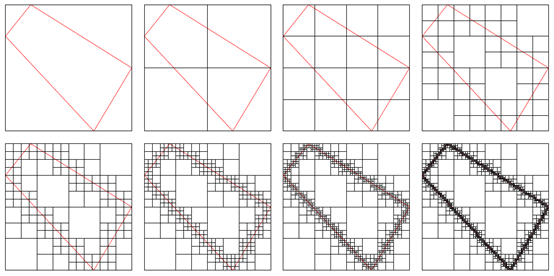
\includegraphics[scale=0.4]{quadtree_octree_netzverfeinerung_kante.png}
%    \item Full Multigrid und Full Approximation Scheme (Nichtlineare Probleme)
%    \item Kombination CG und MG (sogenannter Krylovbeschleunigter MG)
%  \end{itemize}
\end{frame}

\section{Ausblick}\label{sec:Ausblick}
\begin{frame}{Ausblick}
  Ausblick:
  \begin{itemize}[<+(1)->]
    \item Vorkonditionierte CG Verfahren
    \item Mehrgitter für Gitter mit Hindernissen
    \item Lösung der gesamten Navier-Stokes-Gleichungen als System mittels MG
    \item Adaptive Mehrgitter Methode (Adaptive lokale Gitterlevel,
        hierarchische Gitter)
    %\only<5>{
    %\begin{figure}
    %  \centering
    %  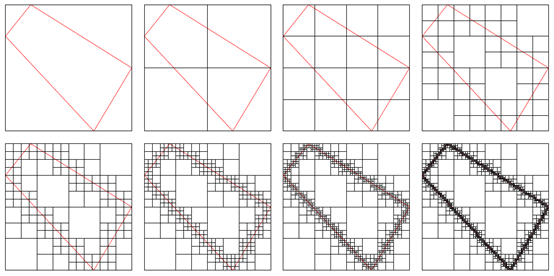
\includegraphics[scale=0.5]{quadtree_octree_netzverfeinerung_kante.png}
    %\end{figure}
    %}
    \only<5>{
      \tikz[overlay, remember picture] {
        \coordinate (picture) at ($(current page.south west)+(8cm,8cm)$);
        \node [below right] at (picture) {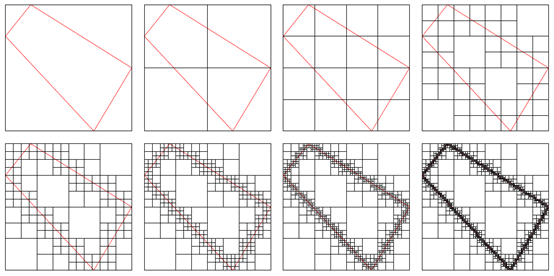
\includegraphics[scale=0.5]{quadtree_octree_netzverfeinerung_kante.png}};
      }%
    }
    \item Full Multigrid und Full Approximation Scheme (Nichtlineare Probleme)
    \only<6>{
      \tikz[overlay, remember picture] {
        \coordinate (picture) at ($(current page.south west)+(8cm,8cm)$);
        \node [below right] at (picture) {
\includegraphics[scale=0.3]{FullMGCycle.png}};
      }%
    }
    \item Kombination CG und MG (sogenannter Krylovbeschleunigter MG)
  \end{itemize}
\end{frame}

\begin{frame}[plain]
  \begin{center}
    \Large \textcolor{simtechred}{ Vielen Dank für die Aufmerksamkeit } \\[2em]
    \normalsize Noch Fragen?
  \end{center}
\end{frame}

\end{document}
